\textit{Runescape} (RS) is a popular \textit{Massively Multiplayer Online Role-Playing Game} (MMORPG) that was first publicly released on January 4'th, 2001 by the video game developer Jagex Limited. Ranked as the 5'th most popular MMORPG in 2020 by several sources, this game's unique mechanisms and game play make it still successful nearly 20 years after it's incarnation \cite{bestreamer:10_most_played_mmorpgs_of_2020, altarofgaming:top_6_most_popular_mmorpgs, thegamer:ranking_the_15_best_mmorpgs}.
On the 20th of November 2012, a total overhaul to the game's combat system - an integral part of gameplay - caused a great divide among it's players. As a result, the game bifurcated into two versions: Runescape 3, and \textit{Old School Runescape} (OSRS). The latter was released on February 22, 2013 and reverted to the old mechanics. The relative player counts over time can be found in Ref.~\cite{misplacedme:relative_player_counts}. OSRS currently contains the majority of players. To limit the already-large scope, this text will only focus on that version.

In typical role-playing fashion, the majority of game play centers around fighting monsters and bosses, training skills, completing quests, playing mini-games, and collecting items. This game is played over the course of months or years. In a few years, there will even be some players who have played for \emph{decades}. As the player base gained a more comprehensive understanding of the game, their mentality has generally shifted from one of discovery to one of \emph{efficiency}. Many tools have been created with the goal of improving player efficiency, optimizing game play, and maximizing success in difficult challenges. %A non-comprehensive list can be found in the \textcolor{red}{appendix [link]}.

There are 23 skills that a player can train \cite{wiki:skills}. A player is rewarded experience for certain actions related to a given skill. For example, cutting an \texttt{Oak Tree} yields 37.5 experience per log chopped. 83 Experience is required to go from level 1 to level 2, while reaching the maximum level of 99 requires 13,034,431 total experience \cite{wiki:experience}. The experience required to level up increases exponentially - hence the drive for efficiency \cite{wiki:experience}. There are several combat skills that directly influence a player's fighting ability. Quests are often completed for the special items, new training methods, and experience rewards they provide. They have skill requirements and often make use of combat in defeating difficult bosses. And so even in this basic overview, the complexity of the interactions and relations between different actions a player can perform becomes apparent.
% Combat is perhaps the most interesting aspect of the game and serves as a dominant focus of this text.

\begin{figure}[h!]
	\centering
	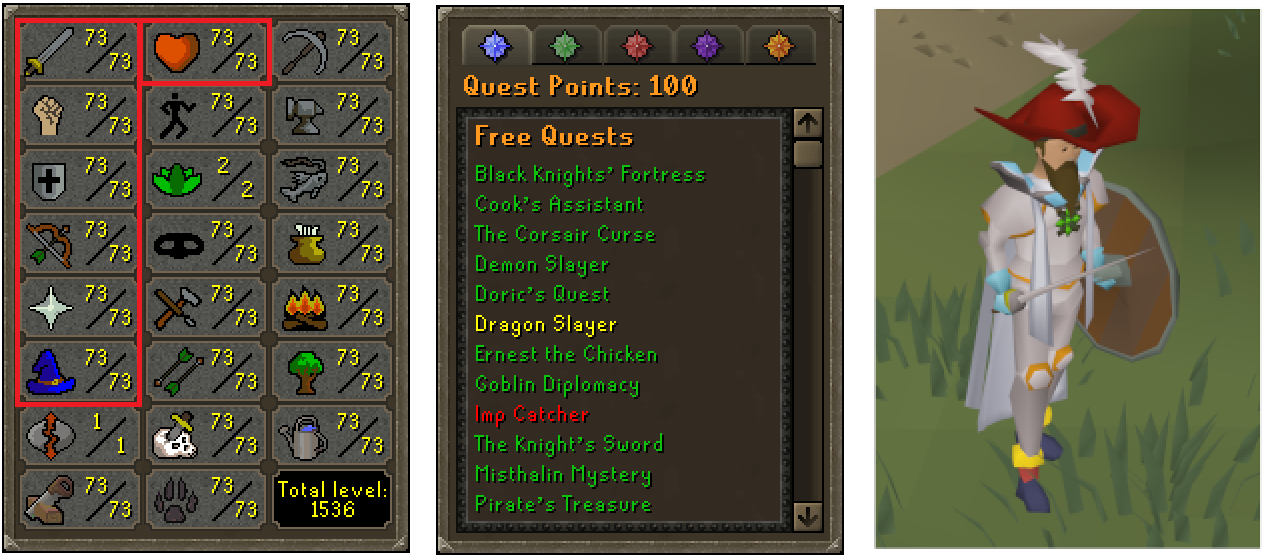
\includegraphics[width=\linewidth]{img/general/skills_quest_player.png}
	\caption{
		Some relevant interfaces/images that play a central role in game play. The skill panel (left) shows the player's levels in the 23 skills along with their total level (Image slightly modified from Ref.~\cite{wiki:skills}). The combat skills, attack, strength, defence, ranged, prayer, magic, and health (in the middle column), are respectively outlined in red. The quest panel (middle) shows the player's quests that are completed, in progress, and not started (green, yellow, and red, respectively. Image from Ref.~\cite{wiki:quests}). A character that a player would control in a 3D world is shown on the right.
	}
	\label{fig:skills_quest_player}
\end{figure}

\newpage
To understand player decisions and optimize them, we will be mathematically modeling the in-game mechanics. A surprising variety of mathematical concepts and techniques will be encountered. Additionally, algorithms derived from computer science are required to solve some of these problems. This serves as an exciting \textit{field} to explore, with some very interesting results and visuals. Some of the details require high level mathematical solutions/descriptions. With the interest of being digestible by a broad audience with varying proficiencies, many arduous solutions are moved to the appendix at the end of each part.
\vspace{2em}
\newline
% This text accompanies an open-source codebase titled \href{https://github.com/Palfore/OSRSmath}{``OSRSmath''} that can be found on Github at \url{https://github.com/Palfore/OSRSmath}. In addition, there is a video series titled ``Optimizing Runescape'' that covers some of these solutions, and can be. Finally, a \href{https://discord.gg/4SXcKQh}{Discord Chat Room} exists for related discussions.
This text accompanies several additional resources:
\begin{enumerate}
	\item Python open-source codebase, \textit{OSRSmath}: \url{https://github.com/Palfore/OSRSmath}.
	\item Video Series, \textit{Optimizing Runescape}: \url{https://www.youtube.com/watch?v=7N9UJX70Z5I&list=PLm3INE_scU5s8NQWmw0fxKtA_6SVxDOc7&ab_channel=Palfore}.
	\item Discord Chatroom: \url{https://discord.gg/4SXcKQh}
\end{enumerate}
